\begin{table}[htbp]
\centering
\caption{Model comparison on the original response scale. Lower RMSE, AIC, and
BIC are better; larger $R^2$ is better. The PINN AIC/BIC values use the same
Gaussian residual criterion as the other fitted mean curves.}
\resizebox{\textwidth}{!}{%
\begin{tabular}{lrrrrrr}
\toprule
Model & RMSE & $R^2$ & AIC & BIC & $p$ & $k$ \\
\midrule
Classical logistic ODE          & 1.4291 & 0.9826 & 165.84  & 171.26  & 2    &
3    \\
Neural ODE                      & 1.0281 & 0.9910 & 2502.20 & 4644.90 & 1185 &
1186 \\
Neural SDE                      & 2.0312 & 0.9649 & 4933.48 & 9217.08 & 2370 &
2371 \\
Deterministic logistic PINN     & 2.8167 & 0.9326 & 4644.90 & 8641.24 & 2211 &
2212 \\
Stochastic logistic PINN drift  & 2.8469 & 0.9311 & 4647.87 & 8646.01 & 2212 &
2213 \\
Stochastic logistic SDE mean    & 3.2324 & 0.9112 & 4659.30 & 8657.44 & 2212 &
2213 \\
\bottomrule
\end{tabular}
}
\label{tab:metrics}
\end{table}

\begin{table}[htbp]
\centering
\caption{Additional stochastic-model diagnostics.}
\begin{tabular}{lrr}
\toprule
Model & 90 percent interval coverage & Mean interval width \\
\midrule
Neural SDE & 0.9333 & 7.3887 \\
Stochastic logistic SDE & 0.8222 & 9.4517 \\
\bottomrule
\end{tabular}
\label{tab:sde-intervals}
\end{table}

\begin{table}[htbp]
\centering
\caption{Estimated logistic PINN inverse-problem parameters. The growth rate
$r$ is on the original time scale.}
\begin{tabular}{lrrr}
\toprule
Model & $r$ & $K$ & $\sigma$ \\
\midrule
Deterministic logistic PINN & 0.035062 & 52.3350 & -- \\
Stochastic logistic PINN/SDE & 0.036806 & 52.2809 & 0.017245 \\
\bottomrule
\end{tabular}
\label{tab:pinn-parameters}
\end{table}

The Neural ODE has the best in-sample interpolation accuracy, with the smallest
RMSE and largest $R^2$. The classical logistic ODE is less flexible, but it
still explains approximately 98.3 percent of the observed variance. Because
AIC and BIC penalize the number of fitted parameters, the two-parameter
logistic model is strongly preferred by these information criteria.

The deterministic logistic PINN and the stochastic logistic PINN drift recover
similar logistic parameters, with $r\approx 0.035$--$0.037$ on the original time
scale and $K\approx 52.3$. Their RMSE values are larger than those of the
classical logistic ODE and the Neural ODE because the PINN objective balances
data fit, initial-condition fit, and a collocation residual rather than
minimizing only the closed-form logistic least-squares objective. The
stochastic logistic SDE mean is less accurate as a fitted mean curve than the
deterministic PINN trajectory, but it provides a process-noise estimate and a
central 90 percent predictive band.

The AIC and BIC values for the neural models should be interpreted as
parameter-penalized residual criteria for the fitted mean curves. They are not
the same as comparing the SDE transition likelihood directly to an exact ODE
likelihood. For the PINNs, these criteria also penalize every neural-network
weight even though the scientific inverse problem has only two or three
physical parameters. Their practical role here is to quantify the tradeoff
between in-sample residual accuracy and model complexity, not to declare a
definitive mechanistic winner.

All comparison figures below were regenerated with the shared plotting style in
\path{src/kefir_models/plot_style.py}. Observed trial markers, fitted mean
curves, predictive bands, legend placement, and the fixed tight canvas are
therefore consistent across the Neural ODE/SDE, logistic PINN, and combined
all-model figures. The step-by-step PNG sequences generated by the plotting
scripts use the same canvas dimensions, so adding a legend entry does not
shift the plotted data region.

\begin{figure}[htbp]
\centering
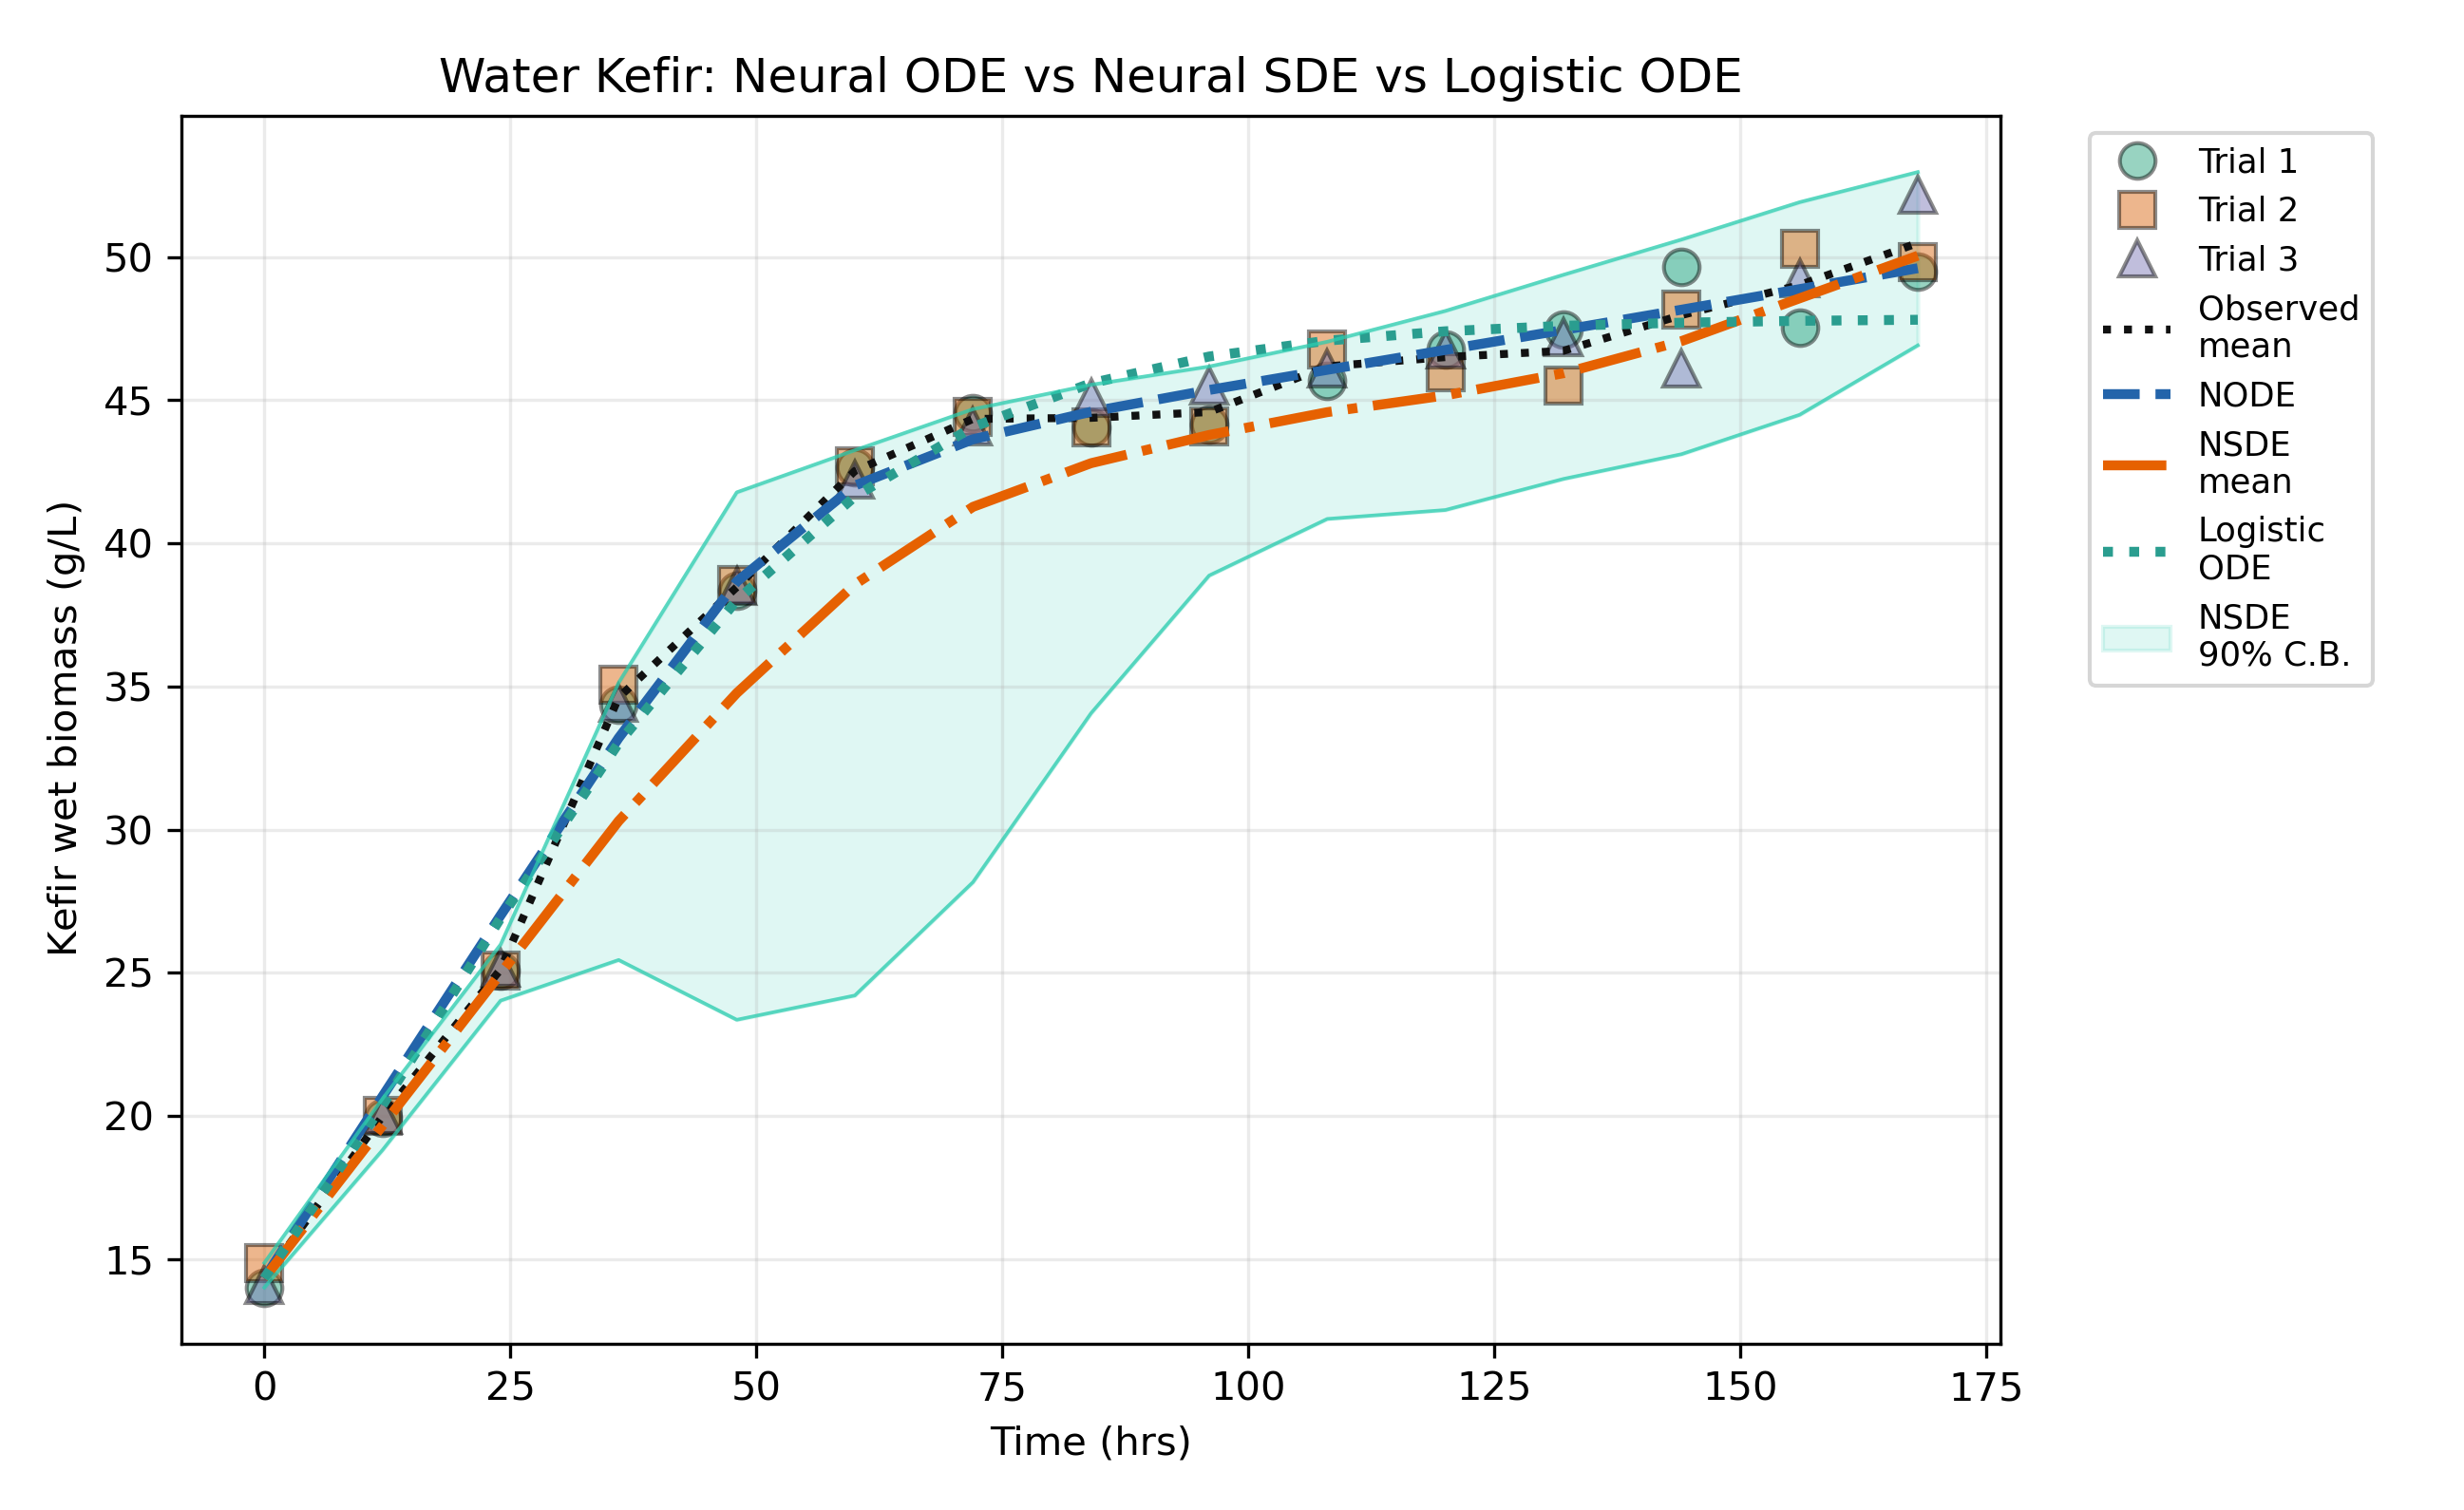
\includegraphics[width=\comparisonfigurewidth]{../results/neural_sde_comparison_outputs/water_kefir_neural_dynamics_comparison.png}
\caption{Observed trial data, the single Neural ODE population curve, fitted
mean trajectories from the comparison models, and the Neural SDE central
90 percent predictive interval. The Neural ODE is fitted as one curve against
all three trial realizations, while the logistic ODE captures the saturating
growth pattern with a much smaller parameter count. The figure uses the shared
fixed-canvas comparison layout.}
\label{fig:fit-comparison}
\end{figure}

\begin{figure}[htbp]
\centering
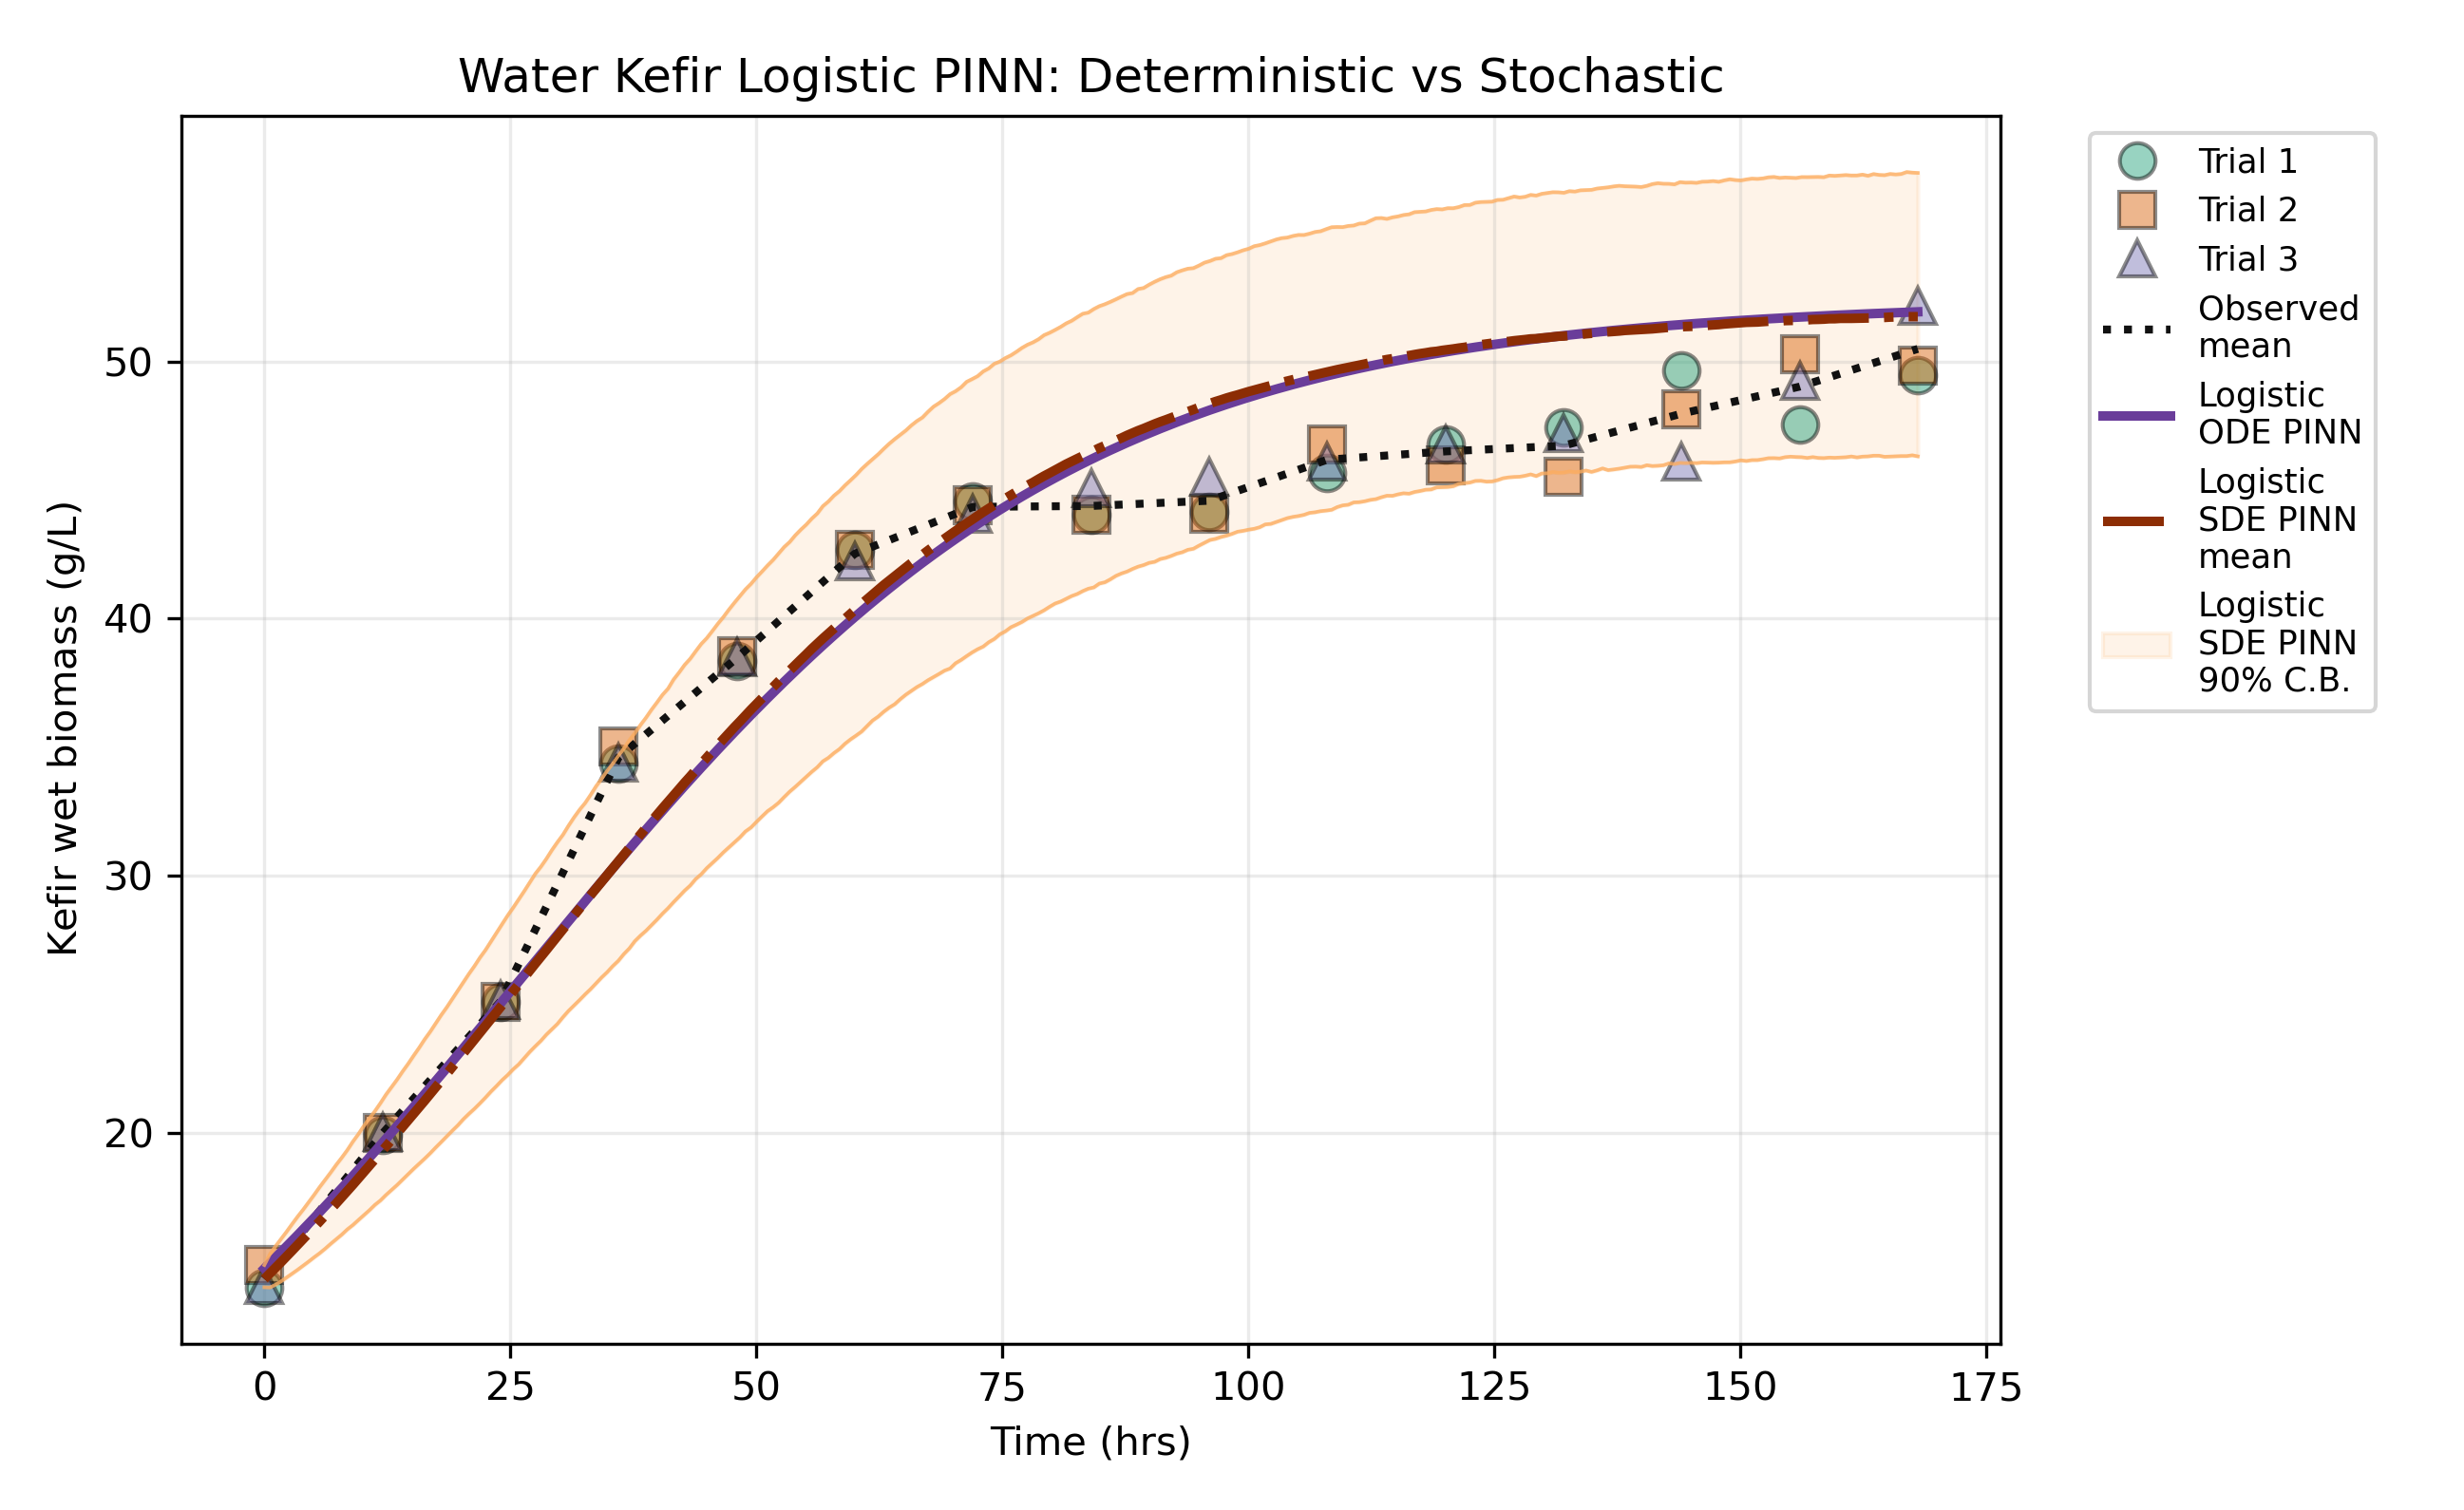
\includegraphics[width=\comparisonfigurewidth]{../results/logistic_pinn_outputs/water_kefir_logistic_pinn_comparison.png}
\caption{Observed trial data, deterministic logistic PINN population
trajectory, stochastic logistic SDE predictive mean, and central 90 percent
predictive interval. The deterministic and stochastic PINNs use the same
three-hidden-layer trajectory architecture and differ by the stochastic
transition-likelihood term used to identify $\sigma$. The line colors and
styles match the all-model comparison.}
\label{fig:logistic-pinn-comparison}
\end{figure}

\begin{figure}[htbp]
\centering
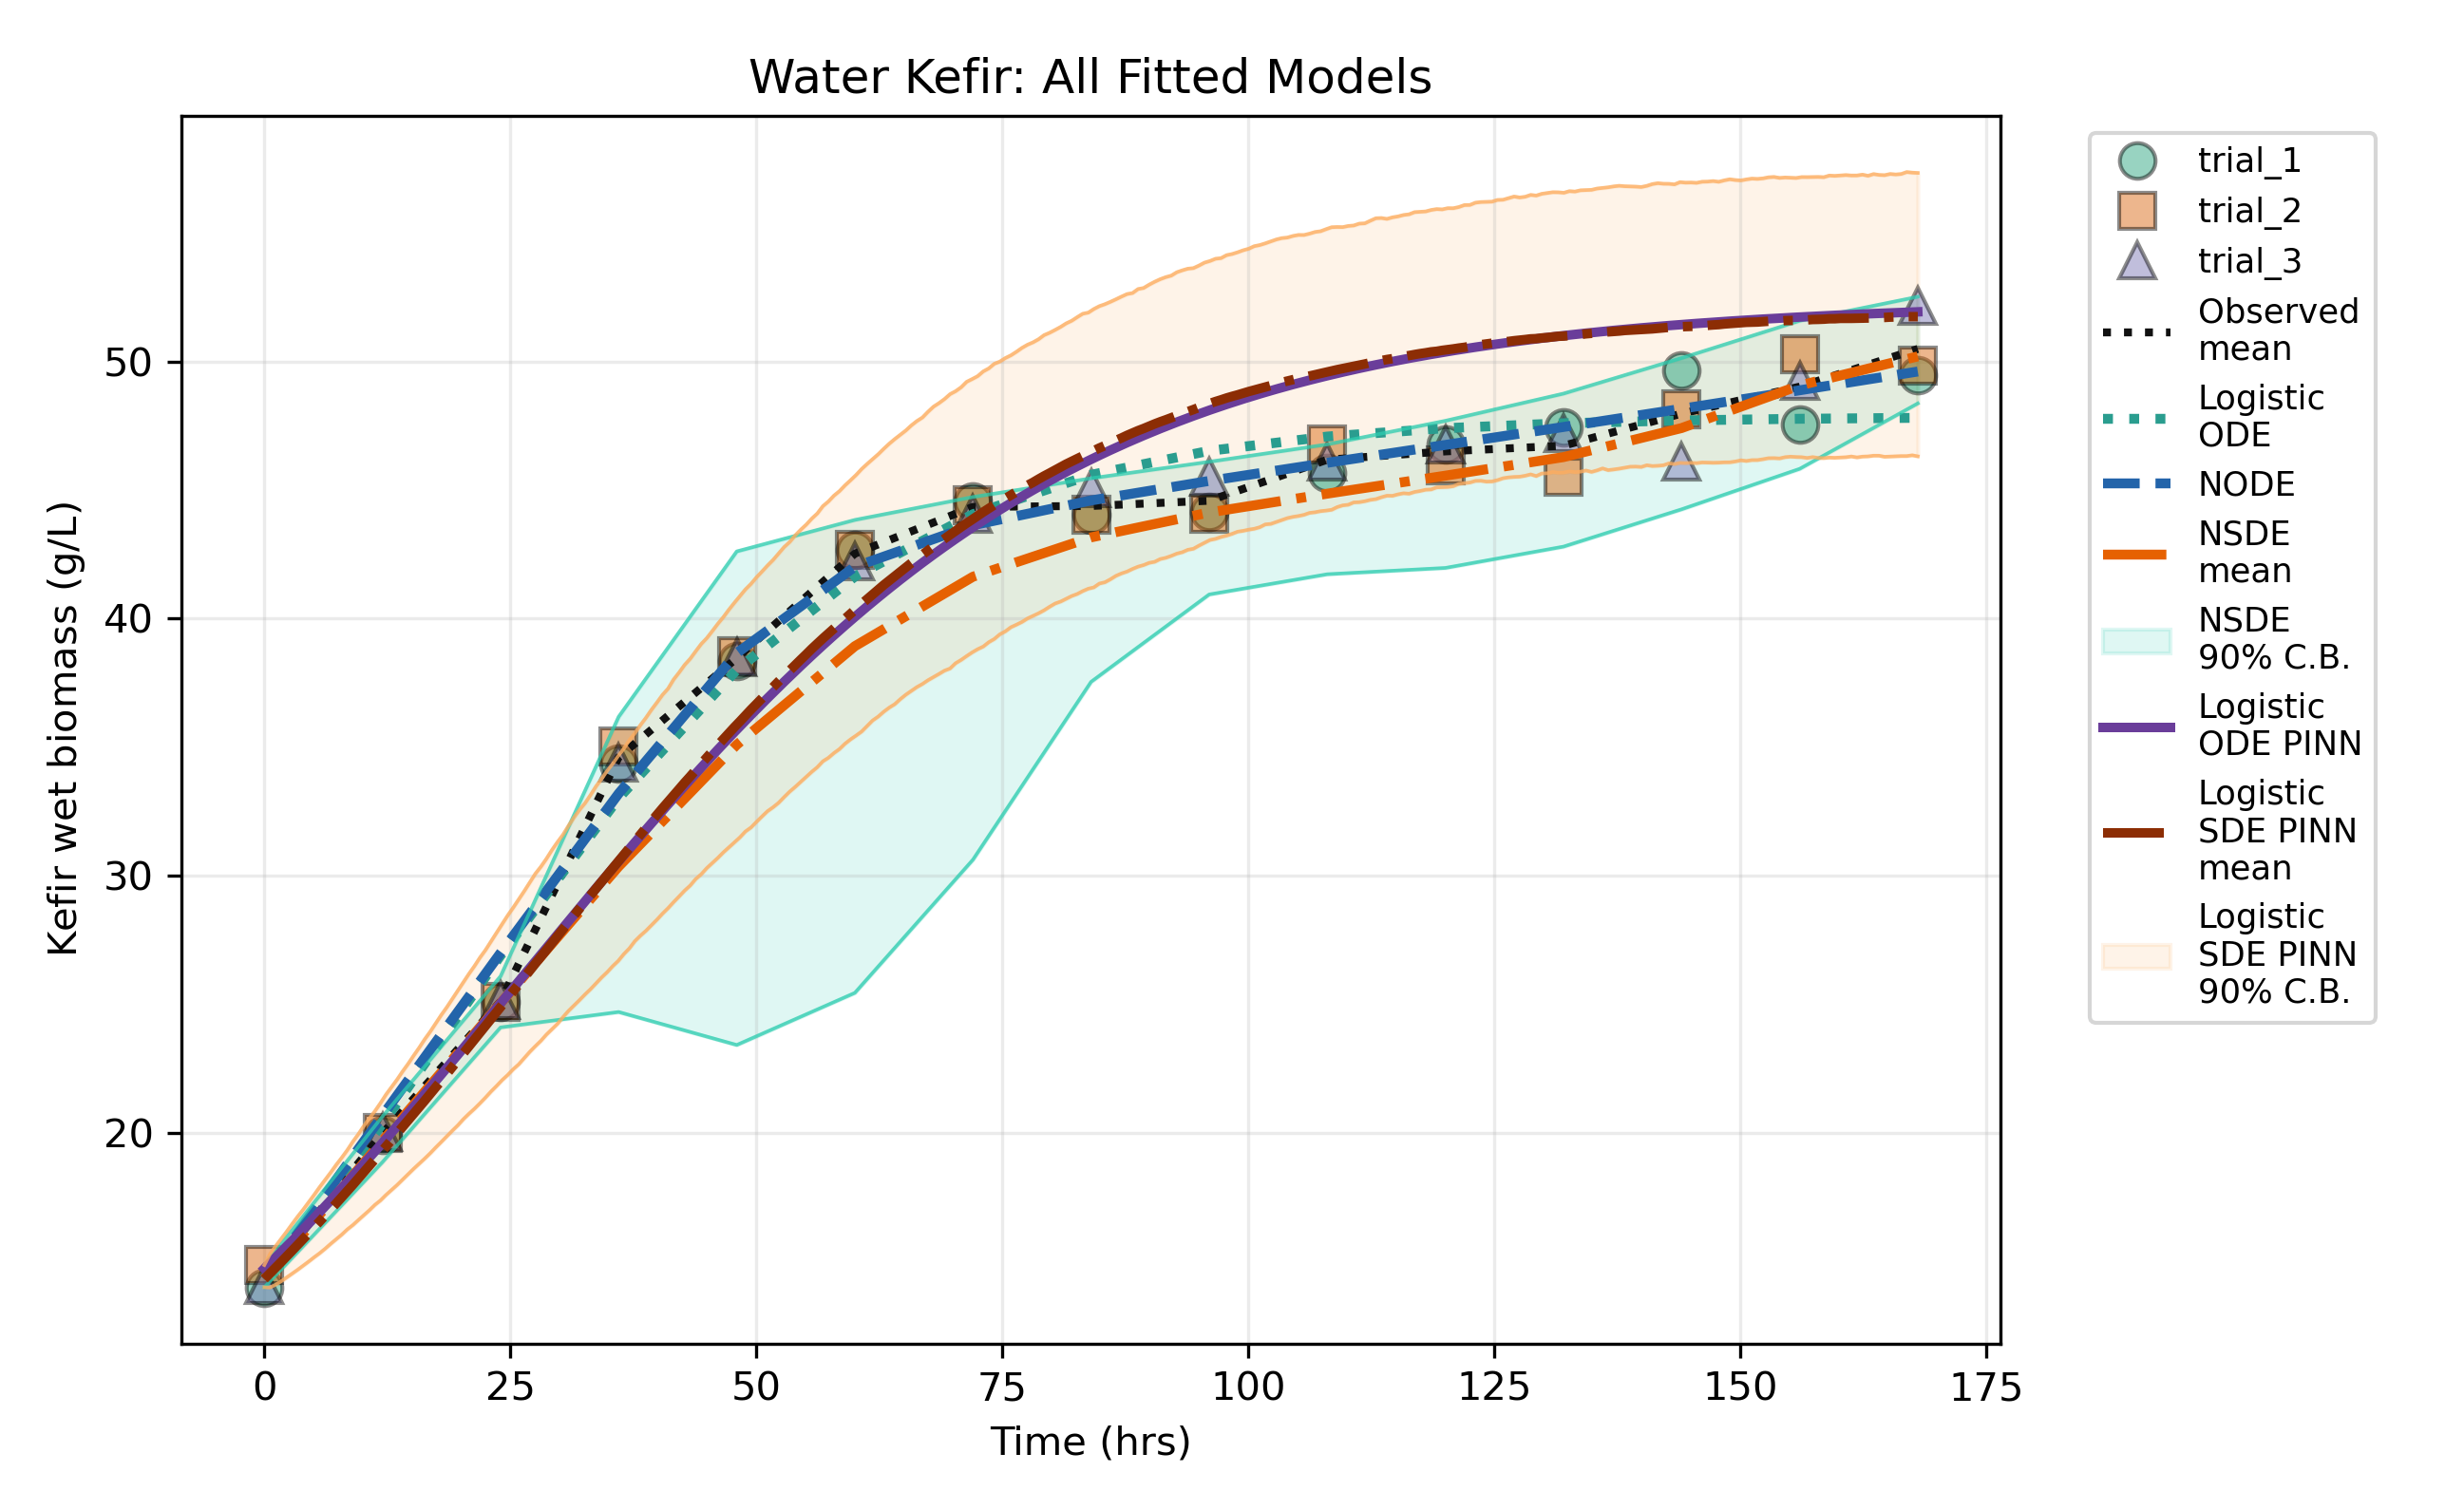
\includegraphics[width=\comparisonfigurewidth]{../results/all_model_comparison_outputs/water_kefir_all_models_comparison.png}
\caption{Combined comparison of the classical logistic ODE, Neural ODE, Neural
SDE, deterministic logistic PINN, and stochastic logistic PINN/SDE outputs. The
plot overlays the two previously separate comparison sequences on a common
original response scale so that fitted mean trajectories and predictive bands
can be visually compared without a layout change between sequence frames.}
\label{fig:all-model-comparison}
\end{figure}

\begin{figure}[htbp]
\centering
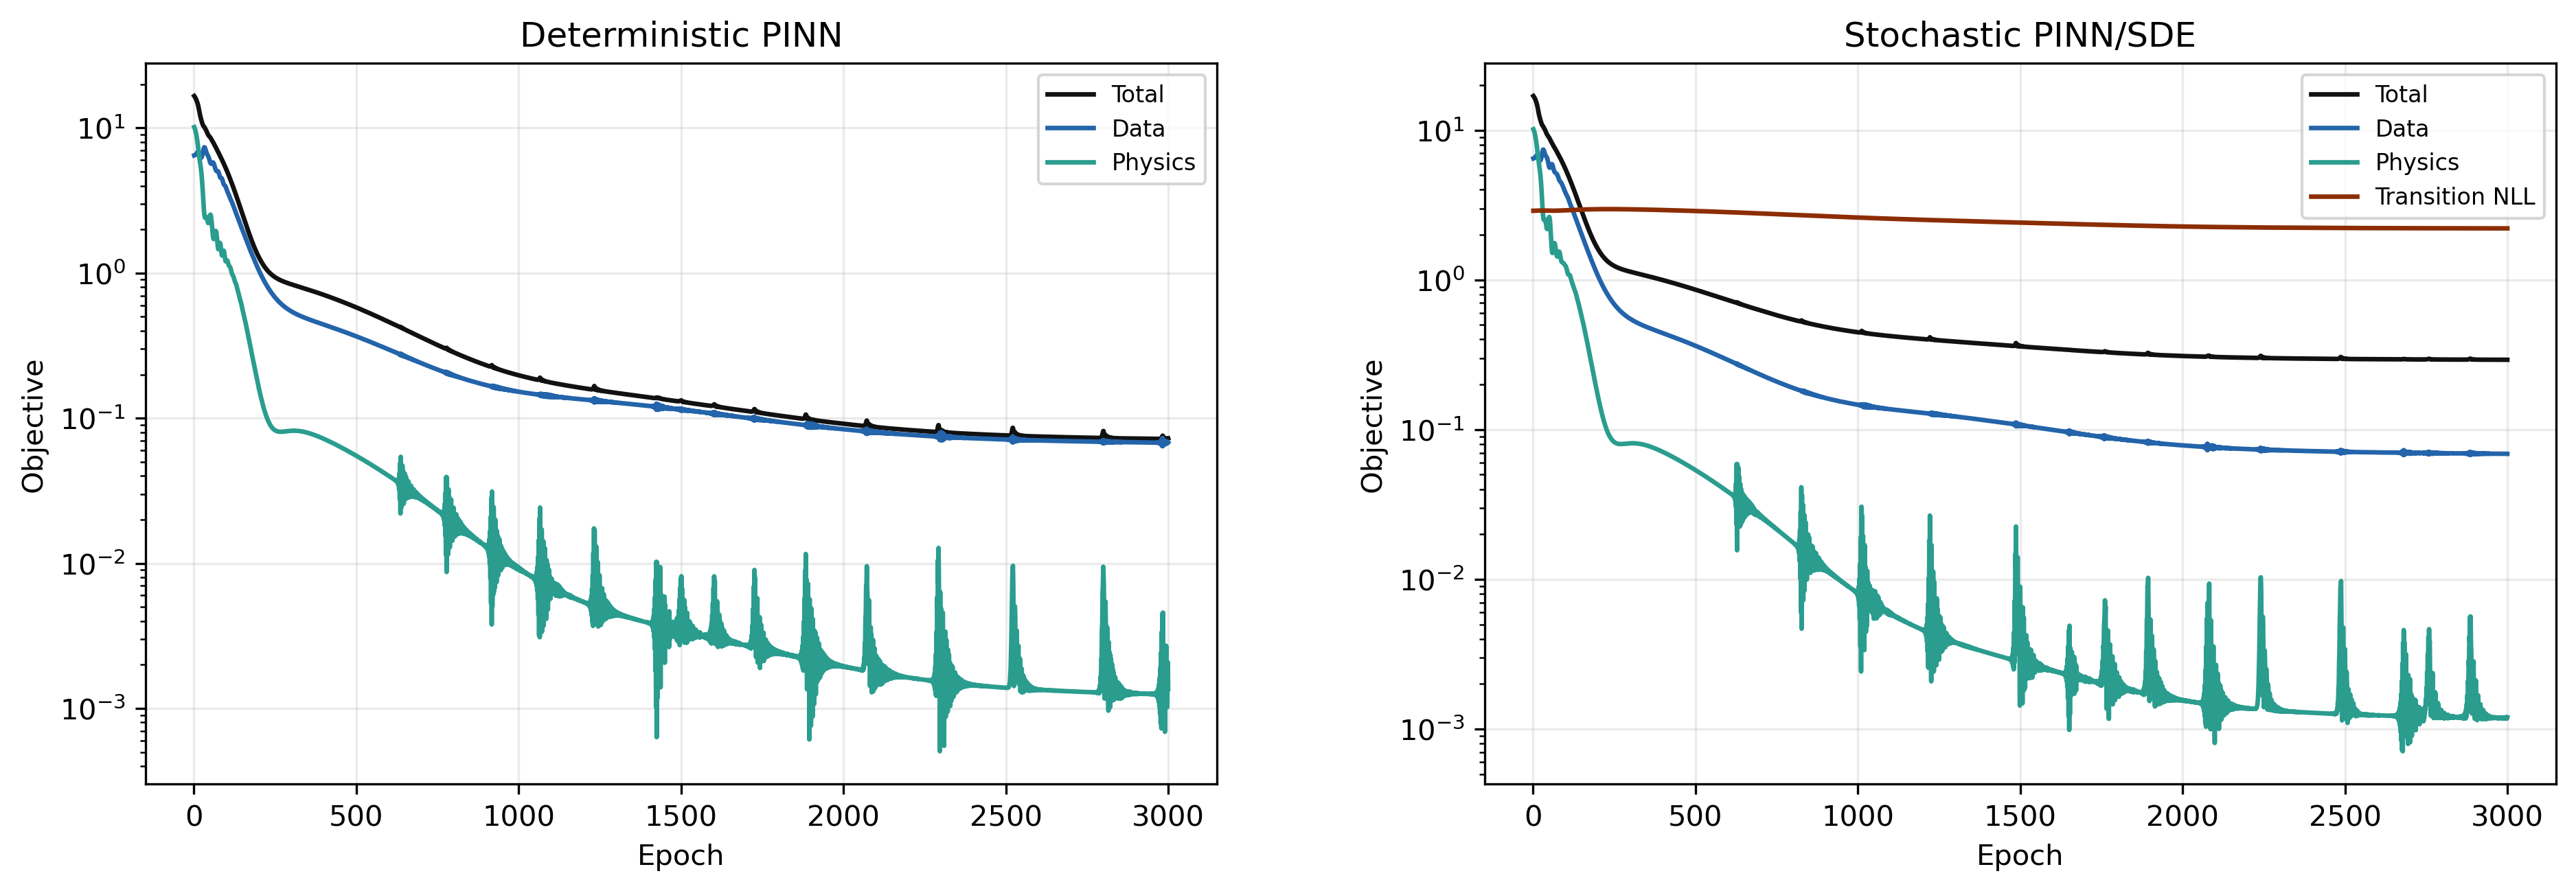
\includegraphics[width=\diagnosticfigurewidth]{../results/logistic_pinn_outputs/water_kefir_logistic_pinn_losses.png}
\caption{Training objectives for the deterministic and stochastic logistic
PINNs. The deterministic objective combines normalized data, initial-condition,
and physics residual terms. The stochastic objective adds the weighted
Euler-Maruyama transition negative log-likelihood.}
\label{fig:logistic-pinn-losses}
\end{figure}

\begin{figure}[htbp]
\centering
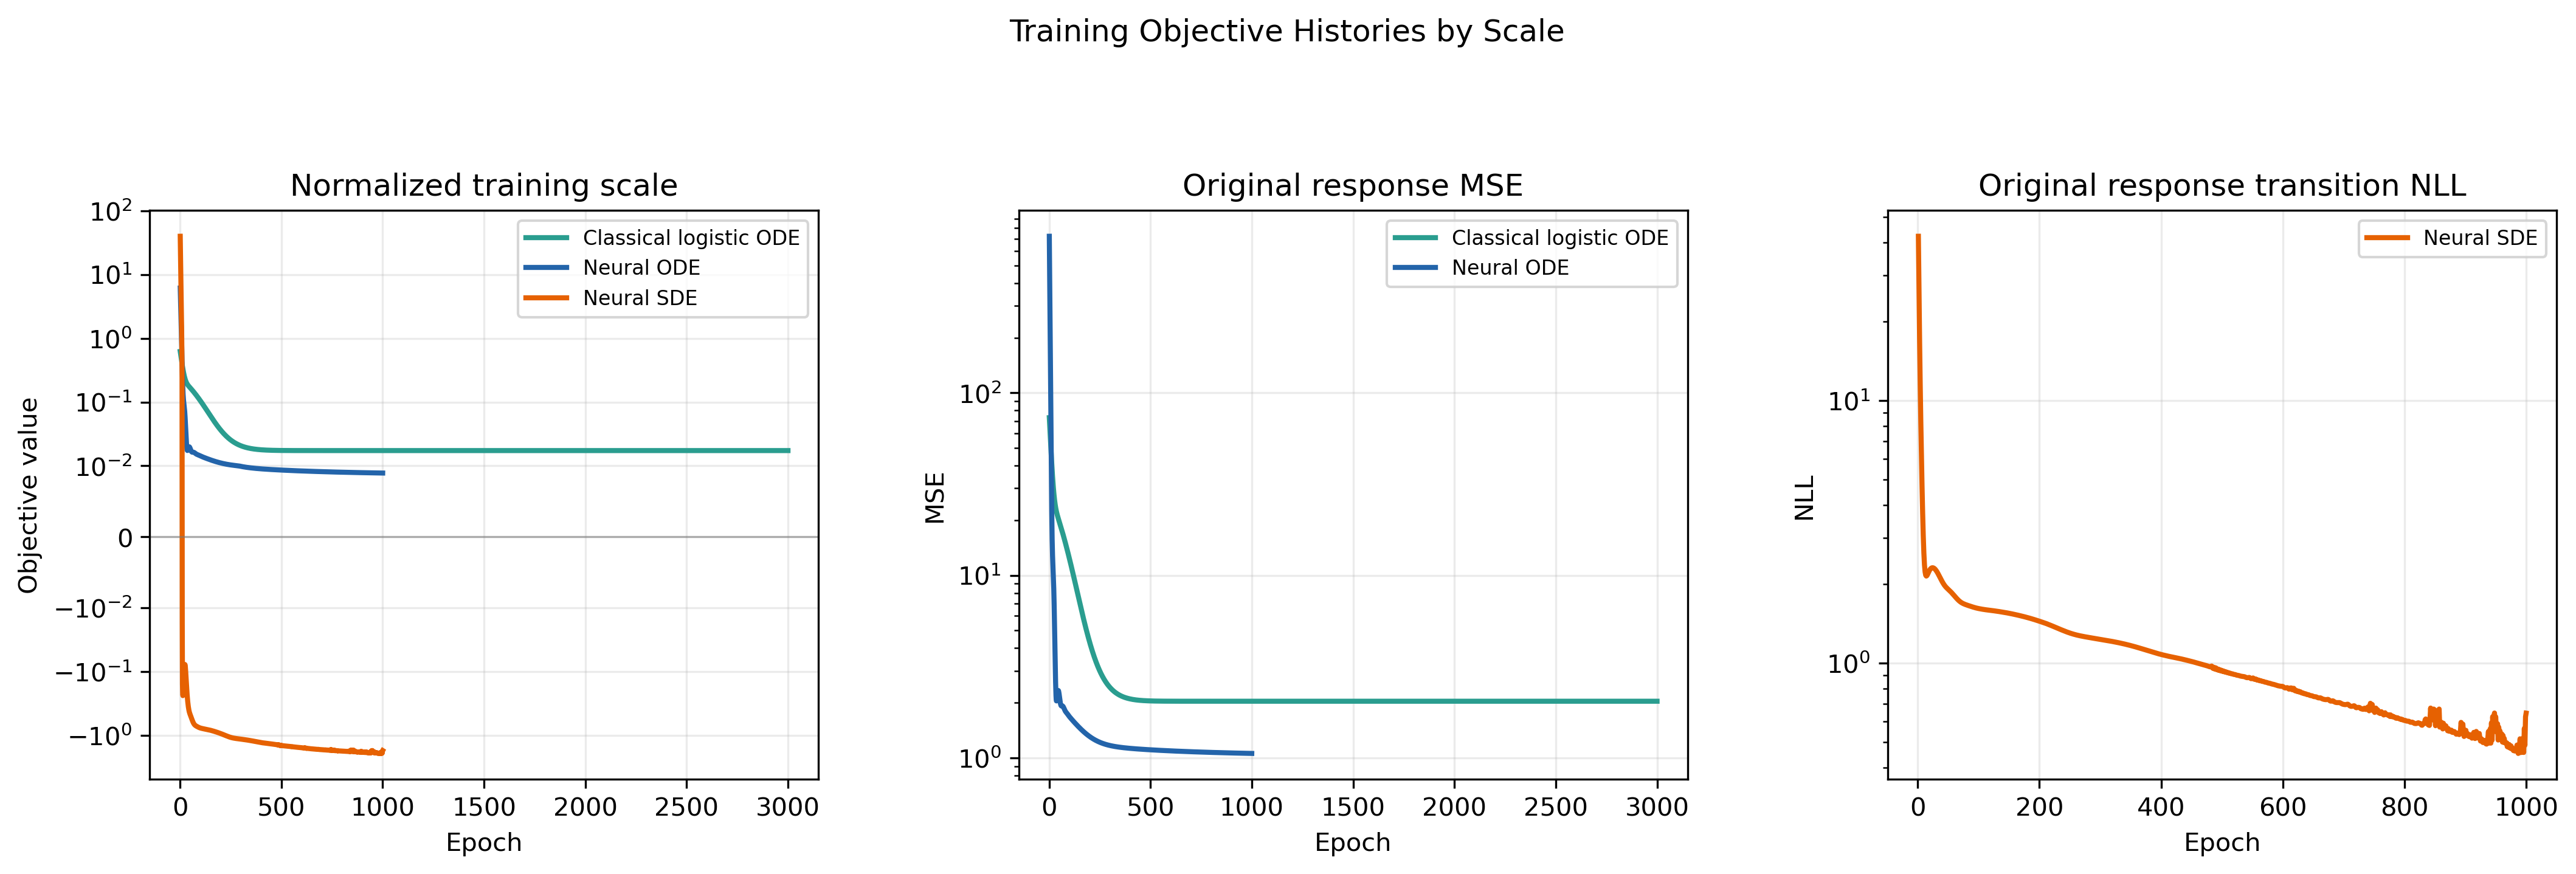
\includegraphics[width=\diagnosticfigurewidth]{../results/neural_sde_comparison_outputs/training_objectives.png}
\caption{Training objective histories from the saved experiment outputs,
re-expressed by scale. The first panel shows the objectives on normalized
training scales, the second panel compares the classical and Neural ODE MSE
histories on the original response scale, and the third panel shows the Neural
SDE transition negative log-likelihood on the original response scale. These
histories are optimization diagnostics, not direct model-comparison metrics,
because MSE and transition likelihood remain different objective types.}
\label{fig:training-objectives}
\end{figure}